\section{04.12.2024}{Wymiar asymptotyczny oraz dowód $\asdim \Z^n=\asdim\R^n= n$}

Niech $X$ będzie zwartą przestrzenią metryczną. Definiujemy wówczas \buff{wymiar $\dim X$} jako najmniejsze $n$ takie, że dla każdego $\epsilon>0$ istnieje skończone pokrycie $U_\epsilon$ przestrzeni $X$ otwartymi zbiorami o średnicy $<\epsilon$ takie, że każdy $x\in X$ należy do $\leq (n+1)$ zbiorów z $U_\epsilon$.

\begin{example}
  $\dim([0,1]\times[0,1])\leq 2$
  Kwadrat możemy rozbić na dowolnie małe cegiełki średnicy $<\epsilon$
  \begin{center}
    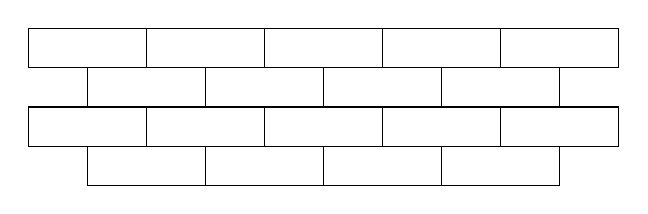
\begin{tikzpicture}
      \begin{scope}
        \draw (0,0)--(6, 0);
        \foreach \i in {0, 1.5, 3, ..., 6} \draw (\i, 0)--(\i, .5);
        \draw (-.75, .5)--(6.75, .5);
        \foreach \i in {-.75, .75, 2.25, ..., 6.75} \draw (\i, .5)--(\i, 1);
      \end{scope}
      \begin{scope}[shift={(0,1)}]
        \draw (0,0)--(6, 0);
        \foreach \i in {0, 1.5, 3, ..., 6} \draw (\i, 0)--(\i, .5);
        \draw (-.75, .5)--(6.75, .5);
        \foreach \i in {-.75, .75, 2.25, ..., 6.75} \draw (\i, .5)--(\i, 1);
      \end{scope}
      \draw (-.75, 1)--(0,1);
      \draw (6, 1)--(6.75,1);

      \draw (-.75, 2)--(6.75, 2);
    \end{tikzpicture}
  \end{center}
  i jako pokrycie wybrać malutkie otoczenia tych cegiełek. Wtedy każdy punkt jest w co najwyżej dwóch zbiorach.
\end{example}

\subsection{Wymiar asymptotyczny}

\begin{definition}{}{}
  Wymiar asymptotyczny $\asdim X$ to najmniejsze $n$ takie, że $(\forall\;R>0)$ istnieje (na ogół nieskończone) pokrycie $U_R$ przestrzeni $X$ zbiorami jednostajnie ograniczonymi (niekoniecznie otwartymi) takimi, że $(\forall x\in X)$ kula $B_R(x)$ należy do co najwyżej $(n+1)$ zbiorów z tego pokrycia.
\end{definition}

\begin{enumerate}
  \item $\asdim X$ jest niezmiennikiem q.i.
  \item $\asdim(\{n^3\;:\;n\in\Z\})=0$
  \item dla $X$ asymptotycznie spójnej, $\asdim X=0$ wtedy i tylko wtedy $X$ jest ograniczona
  \item $\asdim(\Z^n)\leq n$ (patrz: cegłówki wyżej)
  \item $\asdim (X\times Y)\leq \asdim (X)+\asdim(Y)$, ale łatwiej jest pokazać $\asdim(X\times Y)\leq \asdim X+\asdim Y+1$
  \item jeśli $Y\subseteq X$ z obciętą metryką, to $\asdim Y\leq \asdim X$
\end{enumerate}

Yu [1998] pokazał, że jeśli $\asdim G<\infty$, to $G$ spełnia hipotezę Novikova, a w 2003 Roe udowodnił, że $\asdim G<\infty$ $\implies$ $G$ zgrubnie zanurza się w przestrzeni Hilberta.

\begin{center}\slshape\large
Pytanie na dziś: jak pokazać, że $\asdim\Z^n=\asdim\R^n\geq n$?
\end{center}

\subsection{Dowód homologiczny}

Metoda homologiczna będzie polegała na:
\begin{enumerate}
  \item zdefiniowaniu $\asdim_h$ (asymptotyczny wymiar homologiczny)
  \item pokazaniu, że $\asdim_h\Z^n\geq n$
  \item na koniec wystarczy pokazać, że zwykły wymiar asymptotyczny jest nie mniejszy $\asdim \geq \asdim_h$.
\end{enumerate}

\begin{definition}{}{}
  Dla $\epsilon>0$ $q$-wymiarowy $\epsilon$-sympleks w przestrzeni metrycznej $X$ to układ $(x_0,x_1,...,x_q)$ punktów z $X$ (niekoniecznie różnych) takich, że $d_X(x_i, x_j)\leq\epsilon$ dla $0\leq i\neq j\leq q$.
\end{definition}

Określamy w oczywisty sposób $q$-wymiarowe $\epsilon$-łańcuchy, brzegowanie oraz $\epsilon$-homologie $H_q^\epsilon(X)$ [teoria homologii Alexandrowa].

Dla $\epsilon$-łańcucha $U$ w $X$ definiujemy \buff{nośnik $\supp(U)$} jako zbiór wszystkich wierzchołków we wszystkich $\epsilon$-sympleksach z $U$ (mających niezerowy współczynnik).

Dla $\epsilon$-cyklu $z$, jego \buff{$\epsilon$-wypełnieniem} nazywamy dowolny $\epsilon$-łańcuch $w$ taki, że $\partial w=z$.



  $\asdim_h(X)\leq p$ gdy dla każdego $\nu>0$ istnieje $\alpha>0$ (zależna tylko od $X$ i $\nu$) taka, że dla $q\geq p$ dowolny $q$-wymiarowy $\nu$-cykl $\phi$, $\nu$-homologicznie trywialny w $X$, jest także $\alpha$-homologicznie trywialny w swoim nośniku $supp(\phi)$.

  $\asdim_h(X)\geq n$ gdy istnieje $\nu$ takie, że dla każdego $\alpha$ istnieje $(n-1)$-wymiarowy $\nu$-cykl $\nu$-homologii $\phi$ trywialny w $X$ oraz $\alpha$-homologicznie nietrywialny w swoim nośniku.

\begin{definition}{asymptotyczny wymiar homologiczny}{}
  $$\asdim_h(X)=\min \{p\;:\;\asdim_h(X)\leq p\}$$
\end{definition}
% \end{definition}

Można pokazać, że \buff{$\asdim_h$ jest niezmiennikiem q.i.}.

% \subsection{Szkic dowodu, że $\asdim_h(\Z^n)=\asdmin_h(\R^n)\geq n$}

\begin{lemma}{}{}
  $$\asdim_h(\Z^n)=\asdim_h(\R^n)\geq n$$
  % \color{red}Jeśli $\phi$ jest $(n-1)$-wymiarowym $r$-cyklem, który jest $r$-homologicznie trywialny w $\R^n$, to istnieje $\alpha$ taki, że ???
\end{lemma}

\begin{proof}
%% OBRAZEK ZE JEST KWADRAT JAKO Z I JAK GO WYPELNIMY TROJKACIKAMI TO CALOSC JEST W TAKIE, ZE \PARTIAL W=Z
  Niech $\phi$ będzie $(n-1)$-wymiarowym $r$-cyklem, który jest $r$-homologicznie trywialny w $\R^n$. Na obrazku niżej jest taki cykl narysowany dla $r=1$.
  \begin{center}
    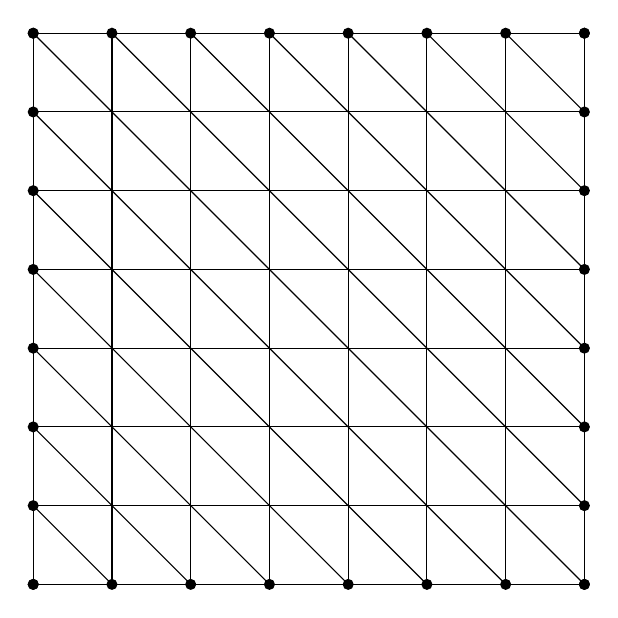
\begin{tikzpicture}
      \foreach \x in {0,..., 7} {
        \fill (\x, 0) circle (2pt);
        \fill (\x, 7) circle (2pt);
        \fill(0, \x) circle (2pt);
        \fill(7, \x) circle (2pt);

        \draw (0,\x)--(7, \x);
        \draw (\x, 0)--(\x, 7);

        \draw (0, \x)--(\x, 0);
      }
      \foreach \x in {1, ..., 7} \draw (7, \x)--(\x, 7);

    \end{tikzpicture}
  \end{center}

  Niech $\alpha\in\R$ będzie dowolne. Twierdzimy, że \textbf{$\phi$ jest $\alpha$-homologicznie nietrywialny w swoim oteczniu}.
  {\large\color{red}NIE ROZUMIEM DOWODU CLAIMU I CO SIE DZIEJE NA OBRAZKU}
\end{proof}
%
% \begin{theorem}{}{}
%   $$\asdim_h(\Z^n)=\asdim_h(\R^n)\geq n$$
% \end{theorem}

\begin{theorem}{}{}
  $$\asdim(X)\geq\asdim_h(X)$$
\end{theorem}

\begin{proof}
  Załóżmy, że $\asdim X=p$. Naszym celem jest pokazanie, że $\asdim_h X\leq p$. 

  Ustalmy $r>0$. Wtedy dla pewnego $q\geq p$ niech $\phi$ będzie $q$ wymiarowym $r$-cyklem $r$-homologicznie trywialnym w $X$. Niech $\mathcal{U}_r$ będzie pokryciem $X$ zbiorami o średnicach $\leq R$ takich, że dowolna kula $B_r(x)$ przecina co najwyżej $(p+1)$ zbiorów z $\mathcal{U}_r$. 

  Rozważmy \buff{$r$-nerw $N$} dla $\mathcal{U}_r$, czyli kompleks taki, że
  \begin{itemize}
    \item $V(N)=\mathcal{U}_r$ wierzchołki odpowiadają zbiorom pokrycia
    \item $U_1,...,U_m\in \mathcal{U}_r$ rozpinają sympleks w $N$ gdy istnieje kula $B_r(x)$ przecinająca $U_1,..., U_m$
    \item $N$ jest $p$-wymiarowym kompleksem symplicjalnym.
  \end{itemize}

  Chcemy teraz przypisać punktom $X$ zbioru z $\mathcal{U}$ i vice versa. Dla każdego $x\in X$ wybierzmy $U_x\in \mathcal{U}_r$ taki, że $x\in U_x$ oraz dla każdego $U\in \mathcal{U}_r$ wybierzmy reprezentanta $z_U\in X$ taki, że $z_U\in U$.

  Przyporządkowanie $x\mapsto U_x$ zmienia $\phi$ na symplicjalny $q$-wymiarowy cykl $\phi_N$ w $N$ symplicjalnie homologiczny zeru. Ponieważ w $N$ nie ma $(q+1)$-sympleksów, to $\phi_N=0$ jako łańcuch.

  Przekształcenie $x\mapsto z_{U_x}$ (złożenie $x\mapsto U_x\mapsto z_{U_x}$) przekształca $\phi$ w $q$-wymiarowy $(r+2R)$-cykl $\phi'$ $(r+2R)$-homologiczny z wyjściowym $\phi$ przez produktowy $(q+1)$ łańcuch $w$. Ponieważ krokiem pośrednim między $\phi$ a $\phi'$ jest $\phi_N=0$, to również $\phi'=0$. W takim razie $w$ jest $(r+2R)$-wypełnieniem $\phi$ o wierzchołkach oddalonych o nie więcej niż $R$ od $\supp\phi$.

  Wierzchołki z łańcucha $w$ leżące poza $\supp\phi$ przesuwamy o nie więcej niż $R$ tak, aby były w $\supp\phi$, dzięki czemu otrzymujemy $(r+4R)$-wypełnienie $\phi$ w $\supp\phi$. W takim razie dla $\alpha=r+4R$ $\phi$ jest $\alpha$-homologicznie trywialny w swoim nośniku. Stąd $\asdim_h(X)\leq p=\asdim(X)$.
\end{proof}

Dostajemy więc 
$$n\geq \asdim(\Z^n)\geq \asdim_h(\Z^n)\geq n$$
czyli $\asdim(\Z^n)=n$.

\subsection{Zgrubna (coarse) niezmienniczość wymiaru asymptotycznego}

\begin{definition}{zgrubne zanurzenie}{}
  Odwzorowanie 
  $$f:(X, d_X)\to (Y, d_Y)$$ 
  jest \buff{zgrubnym zanurzeniem} (coarse embedding), jeśli istnieją dwie funkcje 
  $$\lambda,\mu:\R_+\to \R_+,$$
  które rozbiegają
  $$\lim_{t\to\infty}\lambda(t)=\infty=\lim_{t\to\infty}\mu(t)$$
  oraz dla dowolnych $x,y\in X$ mamy
  $$\lambda(d_X(x,y))\leq d_Y(f(x),f(y))\leq \mu(d_X(x,y)).$$
\end{definition}

Ponadto powiemy, że $f$ jest \buff{zgrubną równoważnością}, jeśli istnieje $L>0$ takie, że $f(x)$ jest $L$-siecią w $(Y, d_Y)$. Równoważnie: istnieje zgrubne zanurzenie $g:Y\to X$ takie, że $f\circ g$ oraz $g\circ f$ są w skończonym dystansie od identyczności.

\begin{example}[m]
  \item Niech $H\leq G$ będzie skończoną podgrupą w skończenie generowanej grupie z generatorami $T\subseteq S$. Metryki $d_T$ oraz $d_S|_H$ na $H$ są zgrubnie równoważne.
  \item Dla przeliczalnie generowanej grupy $(G,S)$ przypisujemy wagi dążące do $\infty$ jej generatorom. Wówczas dowolne dwie ważone metryki słów na $G$ są zgrubnie równoważne.
\end{example}

\begin{fact}{}{}
  Wymiar asymptotyczny jest niezmiennikiem zgrubnej równoważności przestrzeni metrycznych.
\end{fact}

\begin{enumerate}
  \item Jeśli $X$ posiada zgrubne włożenie w $Y$ to $\asdim(X)\leq\asdim(Y)$.
  \item Jeśli $H\leq G$ oraz $H,G$ to skończenie generowane grupy to $\asdim(H)\leq \asdim(G)$
  \item Istnieje naturalne pojęcie $\asdim(G)$ dla przeliczalnie generowalnych grup $G$.
\end{enumerate}

\subsection{Przykład użycia zgrubnej równoważności}

$$Nil=\left\{ \begin{bmatrix}1&a&b\\0&1&c\\0&0&1\end{bmatrix}\;:\;a,b,c\in\Z \right\}-\Z^2\ltimes_Z\Z$$
$$A=\begin{bmatrix}1&1&\\0&1\end{bmatrix}$$

Grupy $Nil$ oraz $\Z^3$ nie są quasi-izometryczne, ale są zgrubnie równoważne poprzez funkcję
$$f:\Z^3\to Nil$$
$$f(a,b,c)=(a,b,c),$$
gdyż dla $x=(a,b,c)$ oraz $y=(a',b',c')$ mamy
$$d_{Nil}(x,y)\leq d_{\Z^3}(x,y)\leq(d_{Nil}(x,y))^2,$$
stąd $\asdim(Nil)=\asdim(\Z^3)=3$.

